% Maintain the consistency.
% Maintain a good writing flow. 

\section{Introduction}\label{sec:introduction}
This document is a documentation of the Virtual Classroom Android App project. The objective of this project is to develop a database application system by applying the theories, methodologies, tools, and technologies learned in Database Management System course]. The app aims to provide a virtual classroom environment for students where they can join in one classroom,
receive class updates, schedule transportation, access class resources, and upcoming events, and view semester information such as course lists, syllabus etc.  


\subsection{Background and Motivation}\label{subsec:bm}

In today's world, online learning has become a popular and necessary approach due to the  COVID-19 pandemic and social distancing norms. The current state of the problem is that traditional physical classrooms are not feasible, and there is a need for an alternative solution. The virtual classroom app aims to address this problem by providing a virtual classroom environment for students. The significance of this solution is that it allows students to continue their education from anywhere, at any time, and it also allows for flexibility in scheduling and learning.

\subsection{Problem Statement}\label{subsec:ps} 
This project aims to address the need for an alternative solution to traditional physical classrooms. The project aims to create a virtual classroom app that allows students to join one classroom, receive class updates, schedule transportation, access class resources, and upcoming events, and view semester information such as course lists, syllabus, etc. The entities in this problem include students, classes, resources, events, and semesters. The relationships between these entities include one-to-many and many-to-many.


\subsection{System Definition}\label{subsec:sd} 

The Virtual Classroom Android App is a computerized system that allows students to join the virtual classroom, receive class updates, schedule transportation, access class resources, and upcoming events, and view semester information such as course lists, syllabus, etc. The system is designed to be easy to use and understand for students, and it allows for flexibility in scheduling and learning.


\subsection{System Development Process}\label{subsec:sdp}

To development this  system ,  we follow the following steps:
\begin{enumerate}
\item Requirement analysis
	\begin{itemize}
		\item[-] In this step, the project team gathers and analyzes the requirements for the database, including the entities, attributes, and relationships needed. The output of this step is a clear understanding of the requirements for the database.
	\end{itemize}

\item Mapping onto a conceptual model (conceptual design)
     \begin{itemize}
     	\item[-] In this step, the project team creates a conceptual model of the database using the ER model. This step includes creating an Entity-Relationship (ER) diagram, which represents the relationships between the entities in the database. The output of this step is a well-designed conceptual model of the database.
     	
     \end{itemize}
     
\item Mapping onto a data model (logical design)
	\begin{itemize}
     	\item[-] In this step, the project team maps the conceptual model onto a logical data model, such as the relational or object model. This step includes creating a logical design of the database, including tables, attributes, and relationships. The output of this step is a well-designed logical data model of the database.
     \end{itemize}
     
\item Normalization
\begin{itemize}
     	\item[-] In this step, the project team normalizes the logical data model to ensure that it is in the 3rd normal form (3NF) and is free from data redundancy and inconsistencies. The output of this step is a normalized database design.
     \end{itemize}
\item System Architecture
\begin{itemize}
     	\item[-] In this step, the project team designs the overall architecture of the system, including the user interface and database design. This step includes creating wireframes and mockups of the app, and determining the overall structure of the app. The output of this step is a detailed system architecture.
     \end{itemize}
     
\item Realization and Implementation (physical design) 
\begin{itemize}
     	\item[-] In this step, the project team codes and develops the database, including the front-end and back-end. This step includes writing code for the app, testing the app, and debugging any errors. The output of this step is a fully functional database.
     \end{itemize}   
    
    
    Each step of the database design process will be a separate section of this document, and the output of each step will be used as the input for the next step.
\end{enumerate}


\begin{figure}[h]

\centering
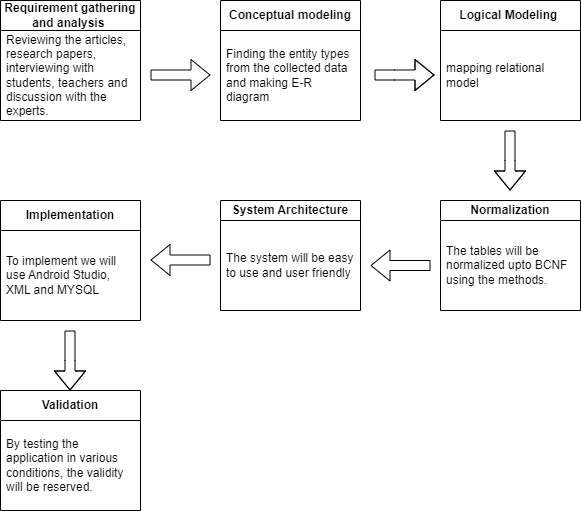
\includegraphics[scale=.5]{sys}

\caption{System Development Process }
\end{figure}


\subsection{Organization} The organization of this document is as follows:

Section~\ref{sec:introduction} gives an overview of the project, including the motivation, problem statement, system definition, and system development process.

Section~\ref{sec:projectmanagement} describes the project management, including the organization of resources, roles of team members, and tools used.

Section~\ref{sec:rga} describes the requirement gathering and analysis process in detail.

Section~\ref{sec:cm} describes the process of creating the conceptual model and ER diagram for the database.

Section~\ref{sec:lm} describes the process of creating the logical data model and mapping the conceptual model onto it.

Section~\ref{sec:norm} describes the process of normalizing the database design.

Section~\ref{sec:sa} describes the system architecture in detail.

Section~\ref{sec:imp} describes the process of coding and implementing the database and android app.

Section~\ref{sec:val} describes the process of testing and validating the database and android app.

Finally, the conclusion and the pointers to the future work are outlined in Section~\ref{sec:cfw}.




\clearpage